\chapter{Evaluation}

\section{The \textit{embeddiogram}, a deep audio feature representation}

The \textit{embeddiogram}, a deep audio feature representation, is derived by applying our pre-trained neural network to sliding windowed segments across the audio signal, generating a sequence of embedding vectors. These relatively low-dimensional embedding vectors collectively form a two-dimensional description of the audio signal's musical content.

Below is a detailed explanation of how we compute the \textit{embeddiogram} from a given audio signal of length $N$. This process comprises loading the audio data, slicing the audio data into windowed segments, processing each window using our pre-trained model to produce a vector per window/time frame, collecting and stacking these embeddings, and finally, normalizing the resulting matrix. 

\begin{enumerate}
\item \textbf{Load the audio data}: The audio data is loaded into memory as a one-dimensional array of length $N$.

\item \textbf{Slice the audio data}: The audio data is segmented into overlapping windows. Each window contains $w$ samples, and consecutive windows are separated by a hop size $h$. This gives a total of $H$ windows, defined as:
\begin{equation}
H = 1 + \left\lfloor \frac{N - w}{h} \right\rfloor
\end{equation}
In the case where $\left( N - w \right) \mod h > 0$, we have $H += 1$ to account for the final, potentially smaller window.

We have conducted experiments using a window duration of 4 seconds (\(w = 4 \times \text{{sr (Hz)}}\)). As a general rule of thumb, this duration corresponds to two 4/4 bars of a piece of music with a tempo where the quarter note equals 120 BPM.

We find this to be a good starting compromise solution, allowing enough time span to capture musical content while not being so large that downsampling reduces the information to an unintelligible vector.

\item \textbf{Process each window}: Each window of audio data is processed independently, passed through the pre-trained neural network, and transformed into an embedding vector. Formally, for each window $w_i$ of audio data, we have:
\begin{equation}
\text{embedding}_i = \text{model}(w_i)
\end{equation}

\item \textbf{Collect the embeddings}: The embedding vectors are collected and stacked together. Each row represents a feature vector for a given time frame to form the \textit{embeddiogram}, denoted as $\text{e}$:
\begin{equation}
\text{e} = \begin{bmatrix} \text{embedding}_1 \\ \text{embedding}_2 \\ \vdots \\ \text{embedding}_H \end{bmatrix}
\end{equation}

\item \textbf{Normalize the \textit{embeddiogram \ref{fig:embeddiogram}}}: The \textit{embeddiogram} is normalized to have a minimum value of 0 and a maximum value of 1 per dimension. The normalization process is given by:
\begin{equation}
E'_{ij} = \frac{e_{ij} - \min(E)}{\max(E) - \min(E)}
\end{equation}
\end{enumerate}

\begin{figure}[ht]
  \centering
  \begin{minipage}[b]{1.0\linewidth}
    \centering
    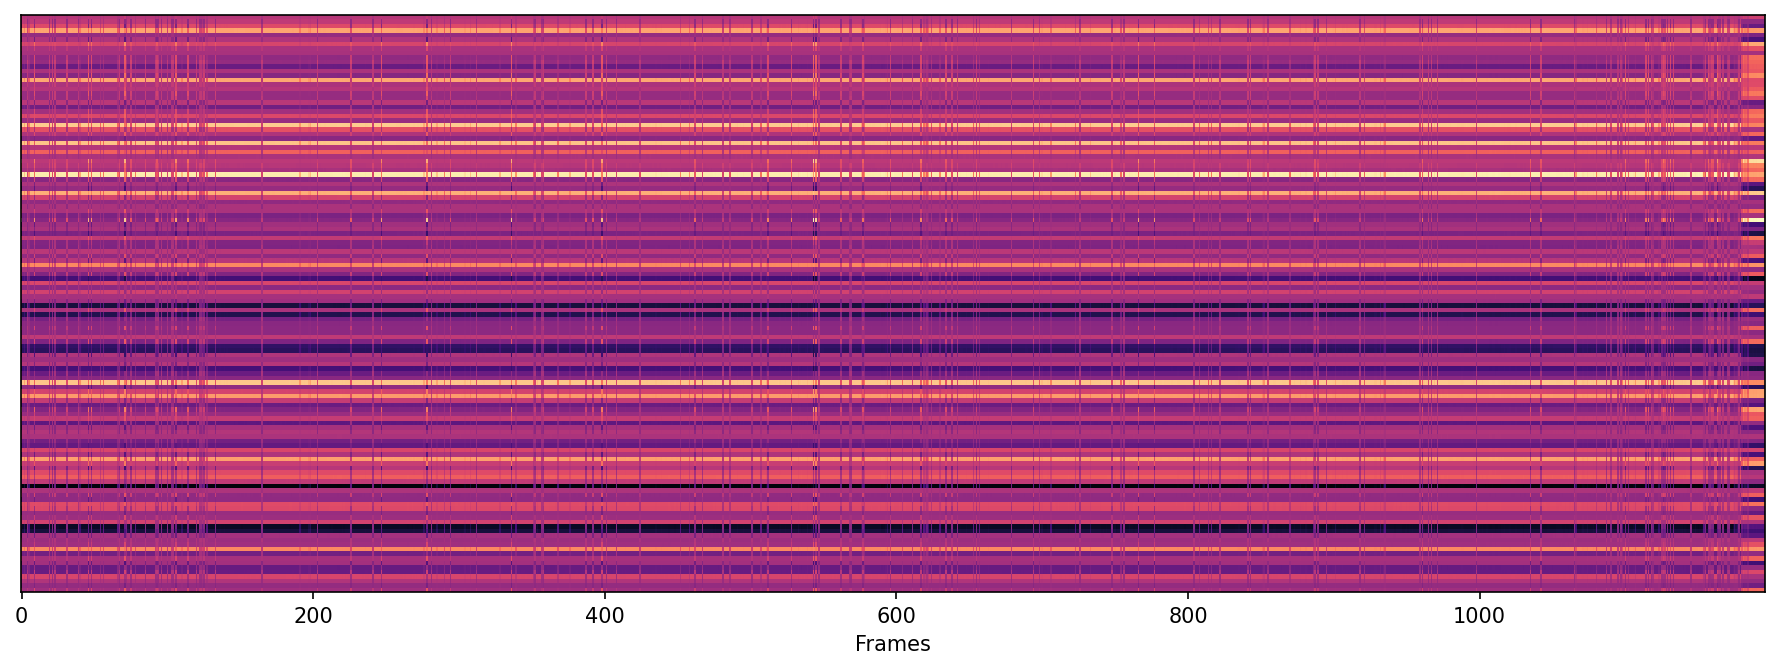
\includegraphics[width=\linewidth]{figures/images/355embeddiogramnormalized.png}
    \caption[Embeddiogram. Track 355 (SALAMI dataset).]{Embeddiogram. Track 355 (SALAMI dataset).}
    \label{fig:embeddiogram}
  \end{minipage}

  \begin{minipage}[b]{1.0\linewidth}
    \centering
    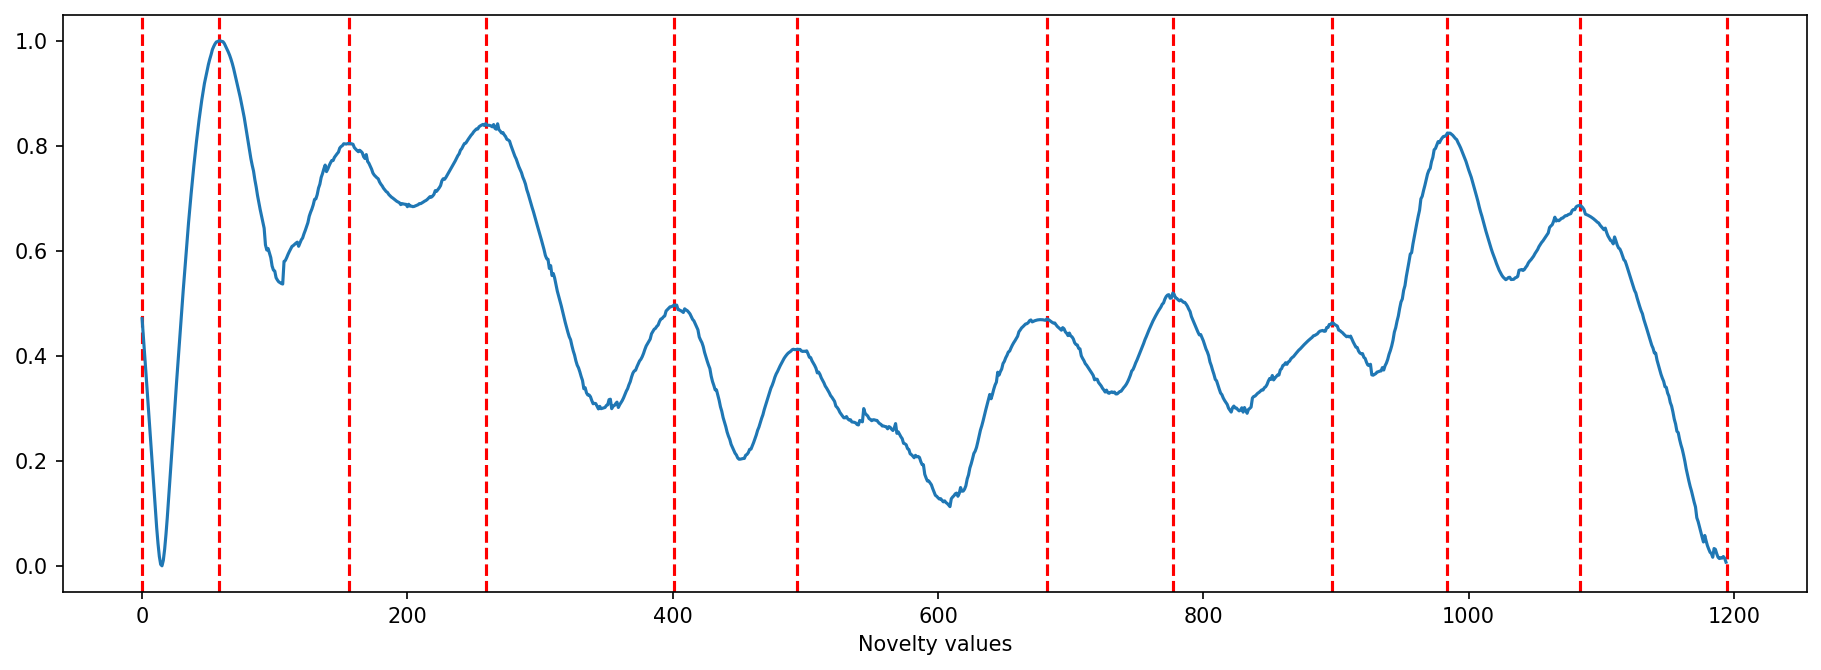
\includegraphics[width=\linewidth]{figures/images/355novelty.png}
    \caption[Novelty curve + peaks. Track 355 (SALAMI dataset).]{Novelty curve and peak detection. Track 355 (SALAMI dataset).}
    \label{fig:novelty}
  \end{minipage}
\end{figure}

\begin{figure}[ht]
    \centering
    \begin{minipage}{0.45\textwidth}
        \centering
        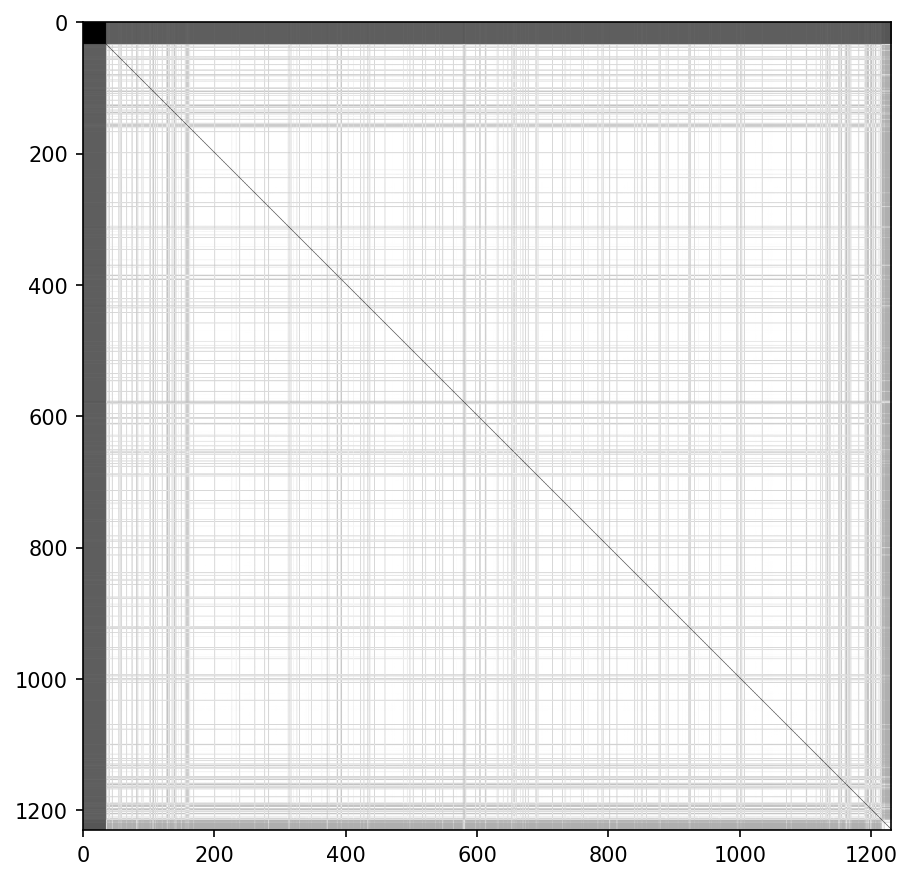
\includegraphics[width=0.9\textwidth]{figures/images/355recurrencematrix.png} % first figure itself
        \caption[Track 355 (SALAMI dataset) Self-similarity matrix]{Self-similarity matrix computation of the embeddiogram. Track 355 (SALAMI dataset).}
        \label{fig:SSM}
    \end{minipage}\hfill
    \begin{minipage}{0.45\textwidth}
        \centering
        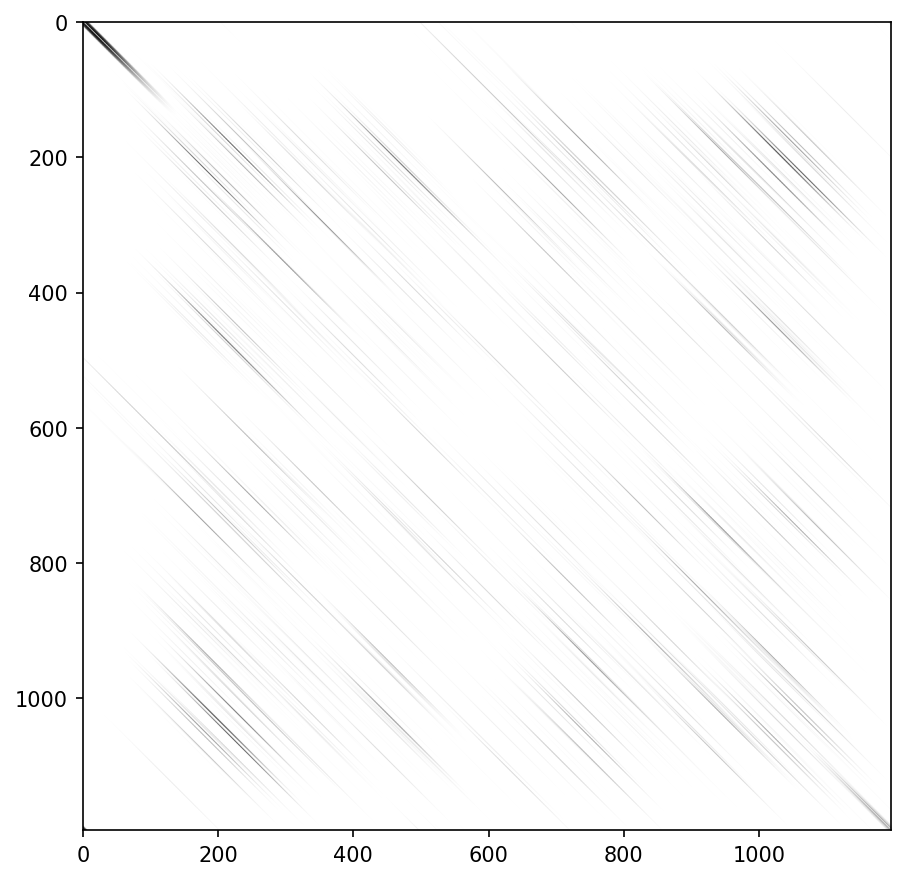
\includegraphics[width=0.9\textwidth]{figures/images/355lagmatrixgaussiansmoothing.png} % second figure itself
        \caption[Track 355 (SALAMI dataset) SSLM computation of the embeddiogram]{Self-similarity lag matrix. Track 355 (SALAMI dataset).}
        \label{fig:SSLM}
    \end{minipage}
    \vfill
    \begin{minipage}{0.45\textwidth}
        \centering
        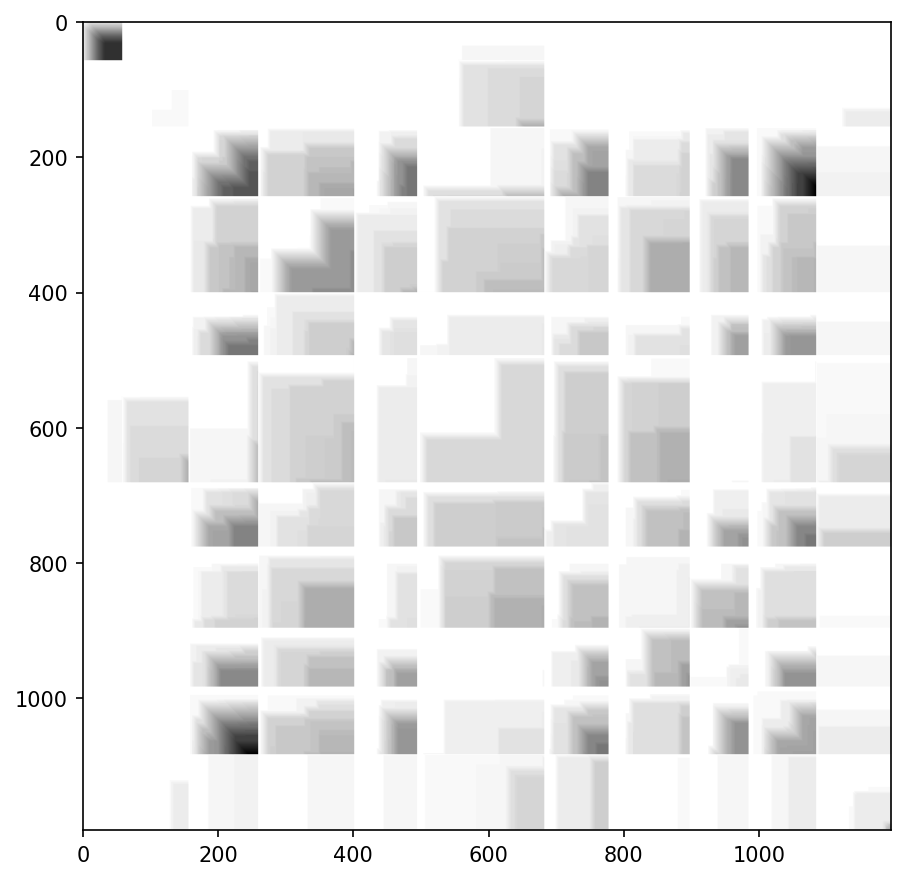
\includegraphics[width=0.9\textwidth]{figures/images/355cumulativematrix.png} % third figure itself
        \caption[Track 355 (SALAMI dataset). Q-matrix]{Cumulative matrix computation of the embeddiogram. Track 355 (SALAMI dataset) .}
        \label{fig:Q}
    \end{minipage}\hfill
    \begin{minipage}{0.45\textwidth}
        \centering
        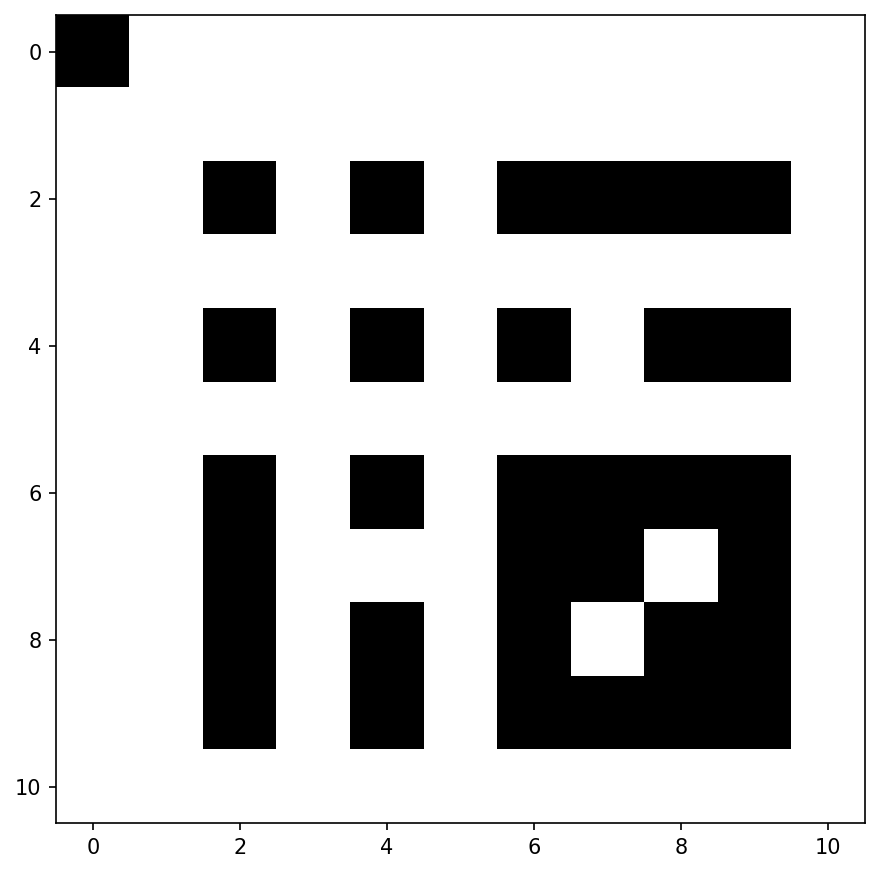
\includegraphics[width=0.9\textwidth]{figures/images/355transitivebinarysimilaritymatrix.png} % fourth figure itself
        \caption[Track 355 (SALAMI dataset). Transitive Binary Similarity Matrix]{Transitive Binary Matrix computation of the embeddiogram. Track 355 (SALAMI dataset).}
        \label{fig:TBSM}
    \end{minipage}
\end{figure}

%%%%%%%%%%%%%%%%%%%%%%%%%

These deep audio features can be a foundation for current state-of-the-art methods, which are expected to receive as input standard traditional audio features. Consequently, they can be processed and manipulated like conventional features as described by \cite{unsuperMSA} and displayed in \ref{fig:novelty}, \ref{fig:SSM}, \ref{fig:SSLM}, \ref{fig:Q}, and \ref{fig:TBSM}. Employing such embeddings in a traditional music segmentation algorithm can achieve state-of-the-art performance \cite{deepfeaturesegment}.

%%%%%%%%%%%%%%%%%%%%%%%%

\section{Music boundary detection as downstream task}

While the usefulness of deep audio embeddings can be evaluated in countless downstream tasks \cite{Li2023MERT:Training, Kim2020OneStrategies}, we have chosen music boundary detection (also known as track segmentation), a subset of music structure analysis (MSA) for its popularity \cite{Smith2013ATask}, complexity, and product-compelling nature. This interdisciplinary field aims to understand the structure of music \cite{Nieto2020Audio-BasedApplications}. Due to subjectivity, ambiguity, and data scarcity, audio-based MSA faces non-solved challenges like boundary placement ambiguity and similarity quantification \cite{NietoPerceptualMusic}.  

%%%%%%%%%%%%%%%%%%%%%%%%%

\section{Evaluation dataset and metrics}

The developed model has been evaluated on the SALAMI dataset \cite{Smith2011DESIGNANNOTATIONS}. The \textit{Structural Analysis of Large Amounts of Music Information} project aims to execute comprehensive structural analyses on a diverse spectrum of music. In contrast to traditional methods, SALAMI segments musical pieces into distinct sections, integrating perceptual, functional, and transcription analyses. Despite certain limitations, this novel approach offers a comprehensive and nuanced understanding of musical structure.

Three primary metrics have been utilized to assess the model performance: Precision, Recall, and F-measure. 

Precision quantifies the proportion of accurately identified boundaries relative to all estimated boundaries to indicate the algorithm's accuracy in boundary detection.

\begin{equation}
\text{Precision} = \frac{\text{True Positives}}{\text{True Positives} + \text{False Positives}}
\end{equation}

On the other hand, Recall measures the proportion of accurately detected boundaries against all reference boundaries, indicating the completeness or sensitivity of the algorithm.

\begin{equation}
\text{Recall} = \frac{\text{True Positives}}{\text{True Positives} + \text{False Negatives}}
\end{equation}

Lastly, the F-measure offers a harmonized view of precision and recall. A widely adopted boundary detection metric, it compares predicted and ground truth boundaries, outputting a score between 0 and 1. This score is calculated as the harmonic mean of Precision and Recall, effectively considering both under-segmentation and over-segmentation. Given the potential inaccuracies inherent in human annotations and prediction errors, the F-measure permits minor deviations between predicted and actual boundaries. Its tolerance threshold can be adjusted, allowing a predicted boundary to be deemed correct if it is within a predefined window of a ground truth boundary \cite{NietoPerceptualMusic, Turnbull2007ABOOSTING}.

We computed the f-measure for each track and then calculated the average rather than aggregating all tracks into a single dataset and calculating the f-measure on this combined set.

\begin{equation}
\text{F-measure} = \frac{2 \times \text{Precision} \times \text{Recall}}{\text{Precision} + \text{Recall}}
\end{equation}

\newpage